%\documentclass[handout]{beamer}
\documentclass{beamer}

\mode<presentation>
{
%\usetheme{Singapore}
%\usetheme{Warsaw}
\usetheme{Malmoe}
\useinnertheme{circles}
%\useoutertheme[footline=empty,subsection=false]{miniframes}
\useoutertheme{infolines}
\setbeamercovered{transparent}
}

\usepackage[english]{babel}
\usepackage[latin1]{inputenc}
\usepackage{bm,textpos,alltt,multirow,ulem}

% font definitions, try \usepackage{ae} instead of the following
% three lines if you don't like this look
\usepackage{mathptmx}
\usepackage[scaled=.90]{helvet}
\usepackage{courier}
\usepackage[T1]{fontenc}

% \usepackage{pgfpages}
% \pgfpagesuselayout{4 on 1}[a4paper,landscape,border shrink=5mm]

\usepackage{xspace}
\makeatletter
\DeclareRobustCommand\onedot{\futurelet\@let@token\@onedot}
\def\@onedot{\ifx\@let@token.\else.\null\fi\xspace}
\def\eg{{e.g}\onedot} \def\Eg{{E.g}\onedot}
\def\ie{{i.e}\onedot} \def\Ie{{I.e}\onedot}
\def\cf{{c.f}\onedot} \def\Cf{{C.f}\onedot}
\def\etc{{etc}\onedot}
\def\vs{{vs}\onedot}
\def\wrt{w.r.t\onedot}
\def\dof{d.o.f\onedot}
\def\etal{{et al}\onedot}
\makeatother

\newcommand{\II}{\mathcal{I}}
\newcommand{\C}{\mathbb{C}}
\newcommand{\D}{\mathcal{D}}
\newcommand{\E}{\mathcal{E}}
\newcommand{\F}{\mathcal{F}}
\newcommand{\I}{\mathcal{I}}
\newcommand{\N}{\mathcal{N}}
\newcommand{\PP}{\mathcal{P}}
\newcommand{\bigO}{\mathcal{O}}
\newcommand{\R}{\mathbb{R}}
\newcommand{\Rz}{\mathcal{R}}
\newcommand{\kb}{\tt}
\newcommand{\blue}{\textcolor{blue}}
\newcommand{\green}{\textcolor{green!70!black}}
\newcommand{\red}{\textcolor{red}}
\newcommand{\brown}{\textcolor{brown}}
\newcommand{\cyan}{\textcolor{cyan}}
\newcommand{\magenta}{\textcolor{magenta}}
\newcommand{\yellow}{\textcolor{yellow}}
\newcommand{\mini}{\mathop{\rm minimize}}
\newcommand{\st}{\mbox{subject to }}
\newcommand{\lap}{\Delta}
\newcommand{\grad}{\nabla}
%\renewcommand{\div}{\nabla \cdot}
\DeclareMathOperator{\divrg}{div}
\def\code#1{{\tt #1}}
\def\shell#1{{\tt \$ #1}}
\newcommand\mtab{\hspace{\stretch{1}}}
\newcommand\ud{\,\mathrm{d}}
\newcommand\bslash{{$\backslash$}}
\newcommand\half{{\frac 1 2}}
\newcommand{\abs}[1]{\left\lvert #1 \right\rvert}
\newcommand{\bigabs}[1]{\big\lvert #1 \big\rvert}
\newcommand{\norm}[1]{\left\lVert #1 \right\rVert}
\newcommand\oneitem[1]{\begin{itemize} \item #1 \end{itemize}}
\newcommand\pp{{\mathfrak p}}
\newcommand\ff{\bm f}
\newcommand\uu{\bm u}
\newcommand\vv{\bm v}
\newcommand\ww{\bm w}
\newcommand\DD{D}
\newcommand{\tcolon}{\!:\!}
\DeclareMathOperator{\sgn}{sgn}
\DeclareMathOperator{\card}{card}
\DeclareMathOperator{\trace}{tr}
\DeclareMathOperator{\sspan}{span}
\renewcommand{\bar}{\overline}
\DeclareMathOperator{\divergence}{div}
\renewcommand\div\divergence


\title{Tightly coupled solvers with loosely coupled software}
\subtitle{Modular linear algebra for multi-physics}

\author{Jed Brown}


% - Use the \inst command only if there are several affiliations.
% - Keep it simple, no one is interested in your street address.
\institute[ETH Z\"urich]
{
  Laboratory of Hydrology, Hydraulics, and Glaciology \\
  ETH Z�rich
}

\date{KAUST 2011-03-27}

% This is only inserted into the PDF information catalog. Can be left
% out.
\subject{Talks}


% If you have a file called "university-logo-filename.xxx", where xxx
% is a graphic format that can be processed by latex or pdflatex,
% resp., then you can add a logo as follows:

% \pgfdeclareimage[height=0.5cm]{university-logo}{university-logo-filename}
% \logo{\pgfuseimage{university-logo}}

\AtBeginSection[]
{
\begin{frame}<beamer>
\frametitle{Outline}
\tableofcontents[currentsection]
\end{frame}
}

% Delete this, if you do not want the table of contents to pop up at
% the beginning of each subsection:
% \AtBeginSubsection[]
% {
% \begin{frame}<beamer>
% \frametitle{Outline}
% \tableofcontents[currentsection,currentsubsection]
% \end{frame}
% }

% If you wish to uncover everything in a step-wise fashion, uncomment
% the following command:

%\beamerdefaultoverlayspecification{<+->}

\begin{document}
\lstset{language=C}
\normalem

\begin{frame}
\titlepage
\end{frame}

\begin{frame}
\frametitle{Outline}
\tableofcontents
% You might wish to add the option [pausesections]
\end{frame}

\section{Throughput for matrices}
\begin{frame}{Bottlenecks of (Jacobian-free) Newton-Krylov}
  \begin{columns}
    \begin{column}{0.4\textwidth}
      \includegraphics[width=1.15\textwidth]{figures/Dohp/EllipRCM}
    \end{column}
    \begin{column}{0.6\textwidth}
      \begin{itemize}
      \item Matrix assembly
        \begin{itemize}
        \item integration/fluxes: FPU
        \item insertion: memory/branching
        \end{itemize}
      \item Preconditioner setup
        \begin{itemize}
        \item coarse level operators
        \item overlapping subdomains
        \item (incomplete) factorization
        \end{itemize}
      \item Preconditioner application
        \begin{itemize}
        \item triangular solves/relaxation: memory
        \item coarse levels: network latency
        \end{itemize}
      \item Matrix multiplication
        \begin{itemize}
        \item Sparse storage: memory
        \item Matrix-free: FPU
        \end{itemize}
      \item Globalization
      \end{itemize}
    \end{column}
  \end{columns}
\end{frame}

\begin{frame}{Hardware capabilities}
  \begin{columns}
    \begin{column}{0.5\textwidth}
      \begin{block}{Floating point unit}
        Recent Intel: each core can issue
        \begin{itemize}
        \item 1 packed add (latency 3)
        \item 1 packed mult (latency 5)
        \item One can include an aligned read
        \item Out of Order execution
        \item Peak: 10 Gflop/s (\texttt{double})
        \end{itemize}
      \end{block}
    \end{column}
    \begin{column}{0.5\textwidth}
      \begin{block}{Memory}
        \begin{itemize}
        \item $\sim 250$ cycle latency
        \item 5.3 GB/s bandwidth
        \item 1 \texttt{double} load / 3.7 cycles
        \item Pay by the cache line (32/64 B)
        \item L2 cache: $\sim 10$ cycle latency
        \end{itemize}
      \end{block}
    \end{column}
  \end{columns}
  \begin{block}{}%<2>{\alert{\Large It's \textbf{all} about the memory hierarchy}}
    \centering
    \includegraphics[width=0.85\textwidth]{figures/OlikerArithmeticIntensity} \\
    \vspace{-1em}
    {\tiny (Oliker et al. 2008)}
  \end{block}
\end{frame}

\begin{frame}[shrink=1]{Memory Bandwidth}
\begin{itemize}
\item Stream Triad benchmark (GB/s): $\bm w \gets \alpha \bm x + \bm y$
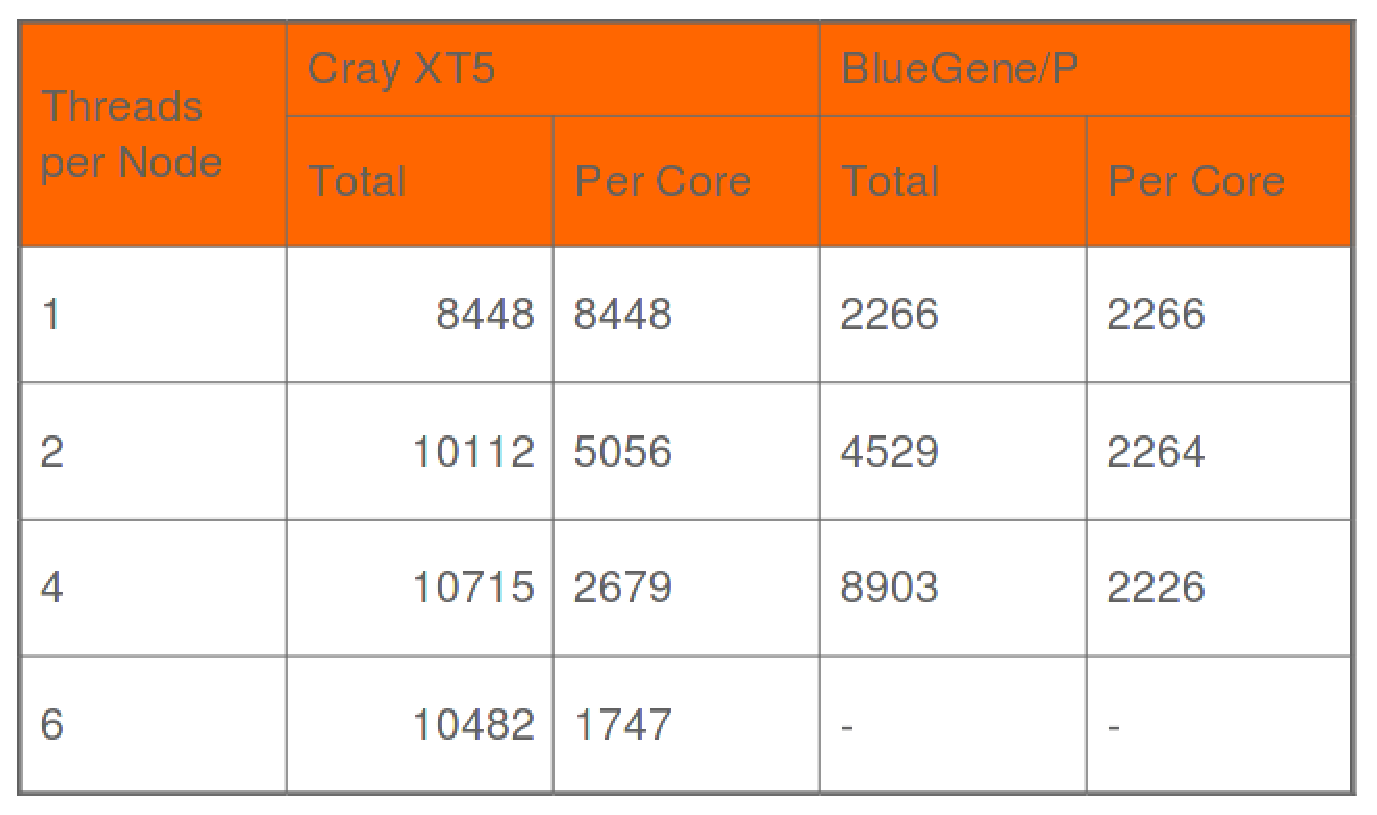
\includegraphics[width=0.8\textwidth]{figures/StreamTriadXT5VsBGP} \\
\item Sparse matrix-vector product: 6 bytes per flop
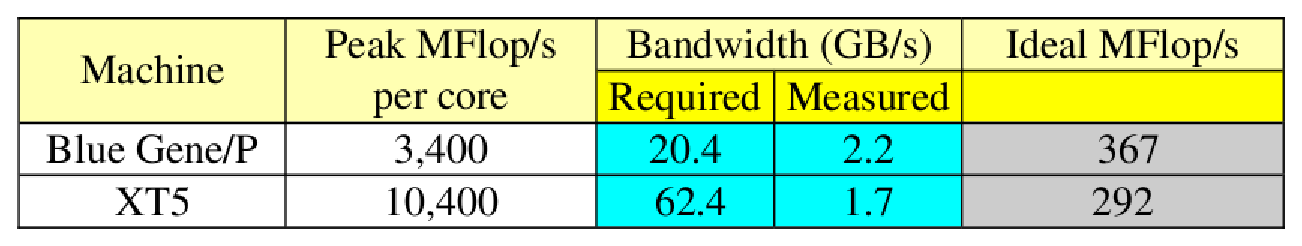
\includegraphics[width=0.8\textwidth]{figures/SparseMatVec} \\
%{\footnotesize (from Dinesh Kaushik)}
\end{itemize}
\end{frame}



\begin{frame}[fragile]{Sparse Mat-Vec performance model}
  \begin{block}{Compressed Sparse Row format (AIJ)}
    For $m \times n$ matrix with $N$ nonzeros
    \begin{itemize}
    \item[ai] row starts, length $m+1$
    \item[aj] column indices, length $N$, range $[0,n-1)$
    \item[aa] nonzero entries, length $N$, scalar values
    \end{itemize}
  \end{block}
\begin{columns}
\begin{column}{0.3\textwidth}
\[y \gets y + A x\]
\end{column}
\begin{column}{0.7\textwidth}
\begin{lstlisting}
  for (i=0; i<m; i++)
    for (j=ai[i]; j<ai[i+1]; j++)
      y[i] += aa[j] * x[aj[j]];
    \end{lstlisting}
  \end{column}
\end{columns}
  \begin{itemize}
  \item One add and one multiply per inner loop
  \item Scalar \code{aa[j]} and integer \code{aj[j]} only used once
  \item Must load \code{aj[j]} to read from \code{x}, may not reuse cache well
  \end{itemize}
\end{frame}

\begin{frame}{Optimizing Sparse Mat-Vec}
  \begin{itemize}
  \item Order unknowns so vector reuses cache (Cuthill-McKee)
    \begin{itemize}
    \item Optimal: $\frac{(2 \text{ flops})(\text{bandwidth})}{\texttt{sizeof(Scalar)} + \texttt{sizeof(Int)}}$
    \item Usually improves strength of ILU and SOR
    \end{itemize}
  \item Coalesce indices for adjacent rows (Inodes)
    \begin{itemize}
    \item Optimal: $\frac{(2 \text{ flops})(\text{bandwidth})}{\texttt{sizeof(Scalar)} + \texttt{sizeof(Int)}/i}$
    \item Can do block SOR (much stronger than scalar SOR)
    \item Default in PETSc, turn off with \code{-mat\_no\_inode}
    \item Requires ordering unknowns so that fields are interlaced, this
      is (much) better for memory use anyway
    \end{itemize}
  \item Use explicit blocking, hold one index per block (BAIJ format)
    \begin{itemize}
    \item Optimal: $\frac{(2 \text{ flops})(\text{bandwidth})}{\texttt{sizeof(Scalar)} + \texttt{sizeof(Int)}/b^2}$
    \item Block SOR and factorization
    \item Symbolic factorization works with blocks (much cheaper)
    \item Very regular memory access, unrolled dense kernels
    \item Faster insertion: \code{MatSetValuesBlocked()}
    \end{itemize}
  \end{itemize}
\end{frame}

\begin{frame}{Performance of blocked matrix formats}
  \centering
  \begin{tabular}{l|c|c|c|c|c|c}
    \multirow{2}{*}{\backslashbox{Kernel}{Format}} & \multicolumn{3}{c|}{Core 2, 1 process} & \multicolumn{3}{c}{Opteron, 4 processes} \\
                      & AIJ & BAIJ & SBAIJ & AIJ  & BAIJ & SBAIJ \\ \hline
    \texttt{MatMult}  & 812 & 985  & 1507  & 2226 & 2918 & 3119  \\
    \texttt{MatSolve} & 718 & 957  & 955   & 1573 & 2869 & 2858  \\
  \end{tabular}
  \bigskip

  {Throughput (Mflop/s) for different matrix formats on Core 2 Duo (P8700) and Opteron 2356 (two sockets). \texttt{MatSolve} is a forward- and back-solve with incomplete Cholesky factors.  The AIJ format is using ``inodes'' which unrolls across consecutive rows with identical nonzero pattern (pairs in this case).}
\end{frame}

\begin{frame}{Optimizing unassembled Mat-Vec}
  \begin{itemize}
  \item High order spatial discretizations do more work per node
    \begin{itemize}
    \item Dense tensor product kernel (like small BLAS3)
    \item Cubic ($Q_3$) elements in 3D can achieve $>70\%$ of peak FPU \\
      (compare to $< 5\%$ for assembled operators on multicore)
    \item Can store Jacobian information at quadrature points \\
      (usually pays off for $Q_2$ and higher in 3D)
    \item Spectral, WENO, DG, FD
    \item Often still need an assembled operator for preconditioning
    \end{itemize}
  \item Boundary element methods
    \begin{itemize}
    \item Dense kernels
    \item Fast Multipole Method (FMM)
    \end{itemize}
  \item<2> \alert{Preconditioning requires more effort}
    \begin{itemize}
    \item Useful to have code to assemble matrices: try out new methods quickly
    \end{itemize}
  \end{itemize}
\end{frame}

\begin{frame}{Power-law Stokes Scaling}
  \centering
  \includegraphics[width=\textwidth]{figures/Dohp/Stokes2} \\
  Only assemble $Q_1$ matrices, ML+PETSc smoothers for elliptic pieces \\
  (easy geometry and coefficients)
\end{frame}

\begin{frame}{What you can do}
  \begin{itemize}
  \item Speak at the most specific language possible
    \begin{itemize}
    \item 3D structural analysis: symmetric block size 3
    \item 3D compressible flow: nonsymmetric block size 5
    \end{itemize}
  \item Order unknowns for cache reuse (low-bandwidth like RCM is good)
  \item Dual order
    \begin{itemize}
    \item Assemble a low-order discretization
    \item Provide matrix-free high-order operator \\
      (FD, ADI, caching at quadrature points)
    \item More robust with SOR and ILU due to $h$-ellipticity
    \item Sometimes Picard linearization has a more compact stencil
    \end{itemize}
  \end{itemize}
\end{frame}

\section{Stiffness}
\begin{frame}[shrink=10]
  \begin{columns}
    \begin{column}{0.5\textwidth}
      \centering
      \includegraphics[width=0.78\textwidth]{figures/MousseauOceanError} \\
      \includegraphics[width=0.78\textwidth]{figures/MousseauOceanTime} \\
      \scriptsize{Shallow water traveling vortex with Coriolis. \\ Moussau et al, 2002.}
    \end{column}
    \begin{column}{0.5\textwidth}
      \includegraphics[width=0.78\textwidth]{figures/KnollSplittingRD} \\
      \scriptsize{Linear reaction-diffusion, split method converges to \\
        the wrong steady state . Knoll et al, 2003.}
      \begin{itemize}\small
      \item CFL too restrictive for explicit
        \begin{itemize}
        \item But hyperbolic systems do not weak scale if you care about phase
        \end{itemize}
      \item Naive semi-implicit has poor accuracy, stability, robustness
      \item Good IMEX exists, but still need to treat stiff part implicitly
      \end{itemize}
    \end{column}
  \end{columns}
\end{frame}

\begin{frame}{Coupled approach to multiphysics}
  \begin{itemize}
  \item Smooth all components together
    \begin{itemize}
    \item Block SOR is the most popular
    \item Vanka smoothers for indefinite problems
    \end{itemize}
  \item Interpolate in a compatible way
  \item Scaling between fields is critical
  \item First-order upwind for transport
  \item Coarse space and subdomain problems should be compatible with inf-sup condition
  \item Open research area
  \end{itemize}
\end{frame}

\begin{frame}{Anisotropy and Heterogeneity}
  \begin{itemize}
  \item Anisotropy
    \begin{itemize}
    \item Semi-coarsening
    \item Line smoothers
    \item Order unknowns so that incomplete factorization ``includes'' a
      line smoother
    \end{itemize}
  \item Heterogeneity
    \begin{itemize}
    \item Make coarse grids align
    \item Strong smoothers
    \item Energy-minimizing interpolants
    \end{itemize}
  \end{itemize}
\end{frame}

\begin{frame}{Splitting for Multiphysics}
  \begin{equation*}
    \begin{bmatrix}
      A & B \\ C & D
    \end{bmatrix}
    \begin{bmatrix}
      x \\ y
    \end{bmatrix}
    =
    \begin{bmatrix}
      f \\ g
    \end{bmatrix}
  \end{equation*}
  \begin{itemize}\item Relaxation:
    \code{-pc\_fieldsplit\_type [additive,multiplicative,symmetric\_multiplicative]}
    \begin{equation*}
      \begin{bmatrix}
        A & \\  & D
      \end{bmatrix}^{-1} \qquad 
      \begin{bmatrix}
        A & \\ C & D
      \end{bmatrix}^{-1} \qquad
      \begin{bmatrix}
        A & \\  & \bm 1
      \end{bmatrix}^{-1}
      \left(
        \bm 1 -
        \begin{bmatrix}
          A & B \\ & \bm 1
        \end{bmatrix}
        \begin{bmatrix}
          A & \\ C & D
        \end{bmatrix}^{-1}
      \right)
    \end{equation*}
    \begin{itemize}
    \item Gauss-Seidel inspired, works when fields are loosely coupled
    \end{itemize}
  \item Factorization: \code{-pc\_fieldsplit\_type schur}
    \begin{align*}
      \begin{bmatrix}
        A & B \\ & S
      \end{bmatrix}^{-1}
      \begin{bmatrix}
        1 & \\ CA^{-1} & 1
      \end{bmatrix}^{-1}, \qquad
      S = D - C A^{-1} B
    \end{align*}
    \begin{itemize}
    \item robust (exact factorization), can often drop lower block
    \item how to precondition $S$ which is usually dense?
      \begin{itemize}
      \item interpret as differential operators, use approximate commutators
      \end{itemize}
    \end{itemize}
  \end{itemize}
\end{frame}

\begin{frame}[shrink=10]{``Physics-based'' preconditioners (semi-implicit method)}
  \begin{block}{Shallow water with stiff gravity wave}
    $h$ is hydrostatic pressure, $u$ is velocity, $\sqrt{gh}$ is fast wave speed
    \begin{gather*}
      h_t - (uh)_x = 0 \\
      (uh)_t + (u^2h + \half gh^2)_x = 0
    \end{gather*}
  \end{block}
  \vspace{-3em}
  \begin{block}{Semi-implicit method}
    Suppress spatial discretization, discretize in time, implicitly for the terms contributing to the gravity wave
    \begin{gather*}
      \frac{h^{n+1} - h^n}{\Delta t} + (uh)_x^{n+1} = 0 \\
      \frac{(uh)^{n+1} - (uh)^{n}}{\Delta t} + (u^2h)_x^{n} + g(h^n h^{n+1})_x = 0
    \end{gather*}

    Rearrange, eliminating $(uh)^{n+1}$
    \[ \frac{h^{n+1} - h^n}{\Delta t} - \Delta t(gh^n h_x^{n+1})_x = -S_x^n \]
  \end{block}
\end{frame}

\begin{frame}[shrink=1]{Delta form}
  \begin{itemize}
  \item Preconditioner should work like the Newton step: $-F(x) \mapsto \delta x$
  \item Recast semi-implicit method in delta form
    \[ \frac{\delta h}{\Delta t} + (\delta uh)_x = -F_0, \quad \frac{\delta uh}{\Delta t} + g h^n (\delta h)_x = -F_1,
    \quad \widehat{J} =
    \begin{pmatrix}
      \frac{1}{\Delta t} & \div \\
      g h^n \nabla & \frac{1}{\Delta t}
    \end{pmatrix}
    \]
  \item Eliminate $\delta uh$
    \[ \frac{\delta h}{\Delta t} - \Delta t(gh^n (\delta h)_x)_x = -F_0 + (\Delta t F_1)_x,
    \quad S \sim \frac{1}{\Delta t} - g \Delta t \div h^n \nabla
    \]
  \item Solve for $\delta h$, then evaluate
    \[ \delta uh = - \Delta t \big[ gh^n (\delta h)_x - F_1 \big] \]
  \item Fully implicit solver
    \begin{itemize}
    \item Is nonlinearly consistent (no splitting error), can be high-order in time
    \item Uses existing code when a semi-implicit method has been implemented
    \item Allows efficient bifurcation analysis, steady-state analysis
    \end{itemize}
  \end{itemize}
\end{frame}

\begin{frame}[shrink=5]{Stokes}
  \begin{block}{Weak form of the Newton step}
    Find $(\uu,p)$ such that
    \begin{align*}
      & \int_\Omega
      \color{red}{(D\vv)^T \big[\eta\bm 1 + \eta' D\ww \otimes D\ww\big] D\uu} \\
      &\qquad\quad - {\color{green!55!black}p \nabla\cdot \vv} - {\color{blue} q \nabla\cdot \uu} = - v\cdot F(\ww) & \forall (\vv,q) \\
    \end{align*}
  \end{block}
  \vspace{-2em}
  \begin{block}{Matrix}
    \vspace{-1.5em}
    \[ \begin{bmatrix}\color{red}{A(\ww)} & {\color{green!55!black} B^T}
      \\ {\color{blue} B} & \end{bmatrix}
    \begin{pmatrix} u \\ p \end{pmatrix}
    = - \begin{pmatrix} F_u(\ww) \\ 0 \end{pmatrix} \]
  \end{block}
  \begin{block}{Block factorization}
    \vspace{-1em}
    \[\begin{bmatrix} A & B^T \\ B & \end{bmatrix} =
    \begin{bmatrix} 1 & \\ BA^{-1} & 1 \end{bmatrix}
    \begin{bmatrix} A & B^T \\ & S \end{bmatrix} =
    \begin{bmatrix} A & \\ B & S \end{bmatrix}
    \begin{bmatrix} 1 & A^{-1}B^T \\ & 1 \end{bmatrix}
    \]
    where the Schur complement is
    \[  S = -B A^{-1} B^T . \]
  \end{block}
\end{frame}

\begin{frame}{Properties of the Schur complement}
  \begin{block}{Block factorization}
    \[
    \begin{bmatrix} A & B^T \\ B & \end{bmatrix} =
    \begin{bmatrix} 1 & \\ BA^{-1} & 1 \end{bmatrix}
    \begin{bmatrix} A & B^T \\ & S \end{bmatrix} =
    \begin{bmatrix} A & \\ B & S \end{bmatrix}
    \begin{bmatrix} 1 & A^{-1}B^T \\ & 1 \end{bmatrix}
    \]
    where
    \[  S = -B A^{-1} B^T . \]
  \end{block}
  \begin{itemize}
  \item $S$ is symmetric negative definite if $A$ is SPD and $B$ has full rank (discrete inf-sup condition)
  \item $S$ is dense
  \item We only need to multiply $B,B^T$ with vectors.
  \item We need preconditioners for $A$ and $S$.
  \item Any definite preconditioner can be used for $A$.
  \item It's not obvious how to precondition $S$, more on that later.
  \end{itemize}
\end{frame}

\begin{frame}[shrink=5]{Preconitioning the Schur complement}
  \begin{itemize}\item $S = -BA^{-1}B^T$ is dense so we can't form it, we need
    $S^{-1}$.\end{itemize}
  \begin{block}{Physics-based commutator: anisotropic pressure diffusion}
    \[ \vv^T A(\ww) \uu \sim \int (D\vv)^T \big[\eta\bm 1 + \eta' D\ww \otimes D\ww\big] D\uu \]
    \begin{itemize}
    \item We would like to find an operator $A_p$ such that
    \[ -S = B A^{-1} B^T \approx BB^T A_p^{-1} =: P_S \]
    so that
    \[ P_S^{-1} = A_p (BB^T)^{-1} \]
    \item Note
      \[ BB^T \sim (-\nabla \cdot)\nabla = - \Delta \]
      corresponds to a Laplacian in the pressure space (multigrid).
    \item If $\eta',\nabla \eta \ll 1$ then $A_p \sim -\eta \Delta$ so $P_S^{-1} = \eta \bm 1$
    \end{itemize}
  \end{block}
\end{frame}

\begin{frame}[shrink=5]{Least squares commutator}
  \begin{itemize}\item Schur complement \[ S = - B A^{-1} B^T \] \end{itemize}
  Suppose $B$ is square and nonsingular.  Then
  \[ S^{-1} = -B^{-T} A B^{-1} . \]
  $B$ is not square, replace $B^{-1}$ with Moore-Penrose pseudoinverse
  \[ B^{\dagger} = B^T(BB^T)^{-1}, \qquad (B^T)^\dagger = (BB^T)^{-1}B .\]  Then
  \[ P_S^{-1} = - (BB^T)^{-1} BAB^T (BB^T)^{-1} . \]
  \vspace{-1em}
  \begin{itemize}
  \item Requires 2 Poisson preconditioners for $(BB^T)^{-1}$ per iteration
  \item Better with scaling, from mass matrices and effective viscosity (Elman et al. 2006, May \& Moresi 2008)
  \item \texttt{-pc\_type fieldsplit -pc\_fieldsplit\_type schur -fieldsplit\_p\_pc\_type lsc -fieldsplit\_p\_lsc\_pc\_type mg}
  \end{itemize}
\end{frame}

\begin{frame}{Unsteady Navier-Stokes}
  % Find $(u,p) \in \VV_D \times \PP$ such that
  % \begin{equation*}
  %   \begin{bmatrix} v \\ q \end{bmatrix}^T J(w) \begin{bmatrix} u \\ p \end{bmatrix} = -F(w) \qquad \forall (v,q) \in \VV_0 \times \PP
  % \end{equation*}
  % \begin{block}{Weak form}
  %   \begin{align*}
  %     \begin{bmatrix} \vv \\ q \end{bmatrix}^T J(\ww) \begin{bmatrix}
  %       \uu \\ p \end{bmatrix} &\sim
  %     \int_\Omega \alert{\rho \vv \cdot (\alpha \uu + \ww \cdot \nabla \uu + \uu \cdot \nabla \ww) + \eta D\vv \tcolon D\uu} \\
  %     &\quad - p \nabla\cdot \vv - q\nabla\cdot \uu
  %   \end{align*}
  % \end{block}
  \begin{block}{Strong form}
    \vspace{-1em}
    \begin{align*}
      J(\ww) \begin{bmatrix} \uu \\ p \end{bmatrix} &\sim \left\{
        \begin{array}{rl}
          \alert{\rho(\alpha \uu + \ww \cdot \nabla\uu + \uu\cdot\nabla\ww) - \eta \nabla^2 \uu} + \nabla p &= -F(w) \\
          \nabla\cdot \uu &= 0
        \end{array} \right.
    \end{align*}
  \end{block}
  \vspace{-1em}
  \begin{block}{Matrix form}
    \vspace{-1em}
    \[
    \begin{bmatrix} \alert{A(w)} & B^T \\ B & \end{bmatrix} =
    \begin{bmatrix} 1 & \\ BA^{-1} & 1 \\ \end{bmatrix}
    \begin{bmatrix} A & B^T \\ & S \\ \end{bmatrix}\qquad S = -BA^{-1}B^T
    \]
  \end{block}
  \vspace{-0.5em}
  \begin{block}{Define $A(w)$ in pressure space}
    \begin{itemize}
    \item Want $P_S = (BB^T) {\color{blue} A_p^{-1}} \approx B A^{-1} B^T,\qquad P_S^{-1} = {\color{blue} A_p} (BB^T)^{-1}$
    \item {\color{blue} $A_p \sim \rho \Big(\alpha p + \ww\cdot \nabla p + p \trace (\nabla\ww)\Big) - \eta \nabla^2 p$}
    \item $p\trace(\nabla\ww)$ term is questionable, not needed for Picard
    \item Almost mesh-independent, weak Reynolds number dependence
    \end{itemize}
  \end{block}
  \vspace{-0.8em}
  {\scriptsize (Silvester, Elman, Kay, Wathen. \emph{Efficient preconditioning of the linearized Navier-Stokes equations for incompressible flow}. 2001) \quad (Elman et al. 2005-2010)}
\end{frame}


\section{Coupling}
\frame{
\frametitle{Flow Control for a PETSc Application}

\begin{center}
\includegraphics[width=4.0in]{figures/SNES/FlowControl}
\end{center}
}

\begin{frame}{Overwhelmed with choices}
  \begin{itemize}
  \item If you have a hard problem, no black-box solver will work well
  \item Everything in PETSc has a plugin architecture
    \begin{itemize}
    \item Put in the ``special sauce'' for your problem
    \item Your implementations are first-class
    \end{itemize}
  \item PETSc exposes an algebra of composition at runtime
    \begin{itemize}
    \item Build a good solver from existing components, at runtime
    \item Multigrid, domain decomposition, factorization, relaxation, field-split
    \item Choose matrix format that works best with your preconditioner
    \item structural blocking, Neumann matrices, monolithic versus nested
    \end{itemize}
  \end{itemize}
\end{frame}
\begin{frame}{Multi-physics coupling in PETSc}
  \begin{columns}
    \begin{column}{0.5\textwidth}
      \tikzstyle{cloud} = [draw, ellipse,fill=red!20, node distance=3cm, minimum height=2em]
      \tikzstyle{block} = [rectangle, draw, fill=blue!20, text width=5em, text centered, rounded corners, minimum height=2em]
      \begin{tikzpicture}
        \node [cloud] (momentum) {Momentum};
        \node [cloud, right of=momentum] (pressure) {Pressure};
        \node<2-> [block, opacity=0.5, fit=(momentum)(pressure), text opacity=0.8] (stokes) {Stokes};
        \node<3-> [cloud, below=2em of momentum] (energy) {Energy};
        \node<3-> [cloud, below=2em of pressure] (geometry) {Geometry};
        \node<4-> [block, opacity=0.4, fit=(stokes)(momentum)(pressure)(energy)(geometry), text opacity=0.8, text height=4em] (ice) {Ice};
        \node<5-> [block, below=2em of ice, minimum width=16em] (bl) {{Boundary \nolinebreak Layer}};
        \node<5-> [block, below=2em of bl, minimum width=16em] (ocean) {Ocean};
        % ]
      \end{tikzpicture}
    \end{column}
    \begin{column}{0.5\textwidth}
      \begin{itemize}
      \item package each ``physics'' independently
      \item solve single-physics and coupled problems
      \item semi-implicit and fully implicit
      \item reuse residual and Jacobian evaluation unmodified
      \item direct solvers, fieldsplit inside multigrid, multigrid inside fieldsplit without recompilation
      \item use the best possible matrix format for each physics \\ (e.g. symmetric block size 3)
      \item matrix-free anywhere
      \item multiple levels of nesting
      \end{itemize}
    \end{column}
  \end{columns}
\end{frame}

\newcommand{\colorA}[1]{{\color{red} #1}}
\newcommand{\colorB}[1]{{\color{green!60!black} #1}}
\newcommand{\colorC}[1]{{\color{blue} #1}}
\newcommand{\colorD}[1]{{\color{magenta!70!black} #1}}
\newcommand{\colorE}[1]{{\color{cyan!70!black} #1}}
\newcommand{\colorF}[1]{{\color{yellow!60!black} #1}}
\newcommand{\colorG}[1]{{\color{red!50!white} #1}}
\begin{frame}{MatNest: a matrix format for field-split}
  \begin{columns}
    \begin{column}{0.65\textwidth}\small
      \begin{equation*}
        \begin{bmatrix}
          \colorA{A_{II}} & \colorA{A_{I\Gamma}}             &                       &                             &                     &   \\
          & \colorB{\alpha M_{\Gamma\Gamma}} &                       & \colorB{- N_{\Gamma\Gamma}} &                       &  \\
          \colorG{G_{II}}      & \colorG{G_{\Gamma I}} & \colorC{B_{II}}       & \colorC{B_{I\Gamma}}        & \colorC{C_{I}^T}    & \colorD{D_I} \\
          \colorG{G_{I\Gamma}} &        \colorG{G_{\Gamma\Gamma}}                          & \colorC{B_{\Gamma I}} & \colorC{B_{\Gamma\Gamma}}   & \colorC{C_{\Gamma}^T} & \colorD{D_\Gamma} \\
          \colorG{G_{Ip}}        &  \colorG{G_{\Gamma p}}                                & \colorC{C_{I}}        & \colorC{C_{\Gamma}}         &                   & \\
          \colorE{\alpha E_I}    & \colorE{\alpha E_\Gamma} & \colorE{F_I} & \colorE{F_\Gamma} & & \colorF{\alpha M_\Theta + J}
        \end{bmatrix}
        \begin{bmatrix}
          x_I \\ x_\Gamma \\ u_I \\ u_\Gamma \\ p \\ \Theta
        \end{bmatrix}
      \end{equation*}
      \begin{itemize}
      \item \colorA{pseudo-elasticity for mesh motion}
      \item \colorB{$(\dot{\bm x} - \bm u)\cdot \bm n = \text{accumulution}$}
      \item \colorG{``just'' geometry}
      \item \colorC{Stokes problem}
      \item \colorD{temperature dependence of rheology}
      \item \colorE{ALE and strain heating in heat transport}
      \item \colorF{thermal advection-diffusion}
      \end{itemize}
    \end{column}
    \begin{column}{0.37\textwidth}
      \begin{itemize}
      \item Blocks stored separately \\
        no-copy access 
      \item \texttt{MatGetSubMatrix} API \\
        looks same as ``normal'' matrices
      \item Nesting can be recursive
      \item Implements standard linear algebra operations
      \end{itemize}
    \end{column}
  \end{columns}
\end{frame}

\begin{frame}
  \alert{\texttt{MatGetLocalSubMatrix(Mat A,IS rows,IS cols,Mat *B);}}
  \begin{itemize}
  \item Primarily for assembly
    \begin{itemize}
    \item \texttt{B} is not guaranteed to implement \texttt{MatMult}
    \item The communicator for \texttt{B} is not specified, \\
      only safe to use non-collective ops (unless you check)
    \end{itemize}
  \item \texttt{IS} represents an index set, includes a block size and communicator
  \item \texttt{MatSetValuesBlockedLocal()} is implemented
  \item MatNest returns nested submatrix, no-copy
  \item No-copy for Neumann-Neumann formats \\ (unassembled across procs, e.g. BDDC, FETI-DP)
  \item Most other matrices return a lightweight proxy \texttt{Mat}
    \begin{itemize}
    \item \texttt{COMM\_SELF}
    \item Values not copied, does not implement \texttt{MatMult}
    \item Translates indices to the language of the parent matrix
    \item Multiple levels of nesting are flattened
    \end{itemize}
  \end{itemize}
\end{frame}


\begin{frame}{Wrap-up}
  \begin{itemize}
  \item Software modularity while retaining access to good solvers
    \begin{itemize}
    \item Reuse single-physics modules
    \item Unintrusive ``special sauce'' (once you figure it out)
    \end{itemize}
  \item Choose the matrix format at runtime, best for your preconditioner
    \begin{itemize}
    \item monolithic, nested, Neumann
    \item scalar or block, symmetric
    \end{itemize}
  \item Break into pieces that are ``understood'', keep some block structure for high throughput
  \end{itemize}
\end{frame}

\end{document}
